%\section{***Linear Regression Analysis under Sets of Conjugate Priors}
%\label{sec:isipta07}

%***short summary of ISIPTA'07 paper??***


\section{A Parameter Set Shape for Strong Prior-Data Agreement Modelling}
\label{sec:boatshape}

%march 2013 notes (technical results)
%Preliminary results
In this section, we will explain an approach for parameter set shapes
that allow for extra precision in case of strong prior-data agreement
as discussed in Section~\ref{sec:concluding-outlook}.
First, we will briefly characterise the novel parametrisation of canoncial conjugate priors this approach relies on.
To keep things simple, we restrict ourselves here for the case of the Beta-Binomial model
(see Section~\ref{sec:beta-binom}),
but the approach is generalisable to arbitrary canonical conjugate priors.%
\footnote{For a more detailed derivation of this parametrisation,
we have to refer to a future publication of Mi\c{k}elis Bickis.}
Then we will suggest a shape in this parametrisation that accomplishes
both \pdc\ sensitivity and `bonus precision' in case of strong prior-data agreement.
We present a parametric description for such a shape
and show that it will indeed lead to the desired properties.

\subsection{A Novel Parametrisation of Canonical Conjugate Priors}
\label{sec:miksworld}

In the parametrisation in terms of $\nz$ and $\yz$, described in Section~\ref{sec:regularconjugates},
a conjugate priors is updated to its respective posterior by a shift in the parameter space,
given by \eqref{eq:canonicalupdate}:
\begin{align*}
\nz &\mapsto \nz + n\,, &
\yz &\mapsto \frac{\nz}{\nz + n} \cdot \yz + \frac{n}{\nz + n} \cdot \frac{\tau(\x)}{n} = \yz + \frac{\tau(\x)-n\yz}{\nz+n}\,.
\end{align*}
We see thus that, while the shift for the $n$ coordinate is the same for all elements $(\nz,\yz)$
in a prior parameter set $\PZ$,
the shift in the $y$ coordinate depends on $\nz$, and the location of $\yz$ itself.
Due to this, the shape of $\PZ$ will change during the update step.

This shape change makes it very difficult to understand the posterior inference properties
of a certain shape of the prior parameter set $\PZ$.
Therefore, a different parametrisation of the canonical priors
in which each coordinate has the same shift in updating would be advantageous.
Then, updating of parameter sets
could be expressed as a shift of the entire set within the parameter space.
%Although interpretation of the shapes may be slightly more difficult due to the,

A parametrisation developed by Mi\c{k}elis Bickis (personal communication) attains*** just that.
He is currently preparing a manuscript elaborating the details of his findings,
and we will present here a preview on the results for the Beta-Binomial case.

In this parametrisation, a canonical prior is represented by a coordinate $(\eta_0,\eta_1)$,
where $\eta_1$ replaces the main prior parameter $\yz$,
while $\eta_0$ is just a different name for $\nz$.
The relation of $(\eta_0,\eta_1)$ to $(\nz, \yz)$ is as follows:
%\begin{equation}
\begin{align}
\label{eq:trafotony}
%\begin{aligned}
\nz &= \eta_0 \,, &
\yz &= \frac{\eta_1}{\eta_0 + 2} + \frac{1}{2}\,.
%\end{aligned}
%\end{equation}
\end{align}

The domain of $\eta_0$ and $\eta_1$ in case of the Beta-Binomial model is
\begin{align}
\label{eq:eta-domain}
\Eta &= \Big\{ (\eta_0,\eta_1) \Big| \eta_0 > -2,\ |\eta_1| < \frac{1}{2}(\eta_0 + 2) \Big.\Big\}\,,
\end{align}

and the update step in terms of $\eta_0$ and $\eta_1$ is given by
\begin{equation}
\label{eq:eta-update}
\begin{aligned}
\eta_0\un &= \eta_0\uz + n\,, \\
\eta_1\un &= \eta_1\uz + \frac{1}{2}(s - (n-s)) = \eta_1\uz + s - \frac{n}{2}\,,
\end{aligned}
\end{equation}
where we denote prior parameters with superscript ${}\uz$, and posterior parameters with superscript ${}\un$,
while $s$ is the number of successes in the $n$ Bernoulli trials.
A `success' in a Bernoulli trial thus
leads to step of $1$ in the $\eta_0$ direction and of $+\frac{1}{2}$ in the $\eta_1$ direction,
while a `failure'
leads to step of $1$ in the $\eta_0$ direction and of $-\frac{1}{2}$ in the $\eta_1$ direction.%
\footnote{As in Section~\ref{sec:isipta11}, we  
will often consider $s$ as a a real-valued observation in $[0,n]$
because the continuous representation is convenient for our discussions,
keeping in mind that in reality it can only take on integer values.}

\begin{figure}  %trim=l b r t
\centering
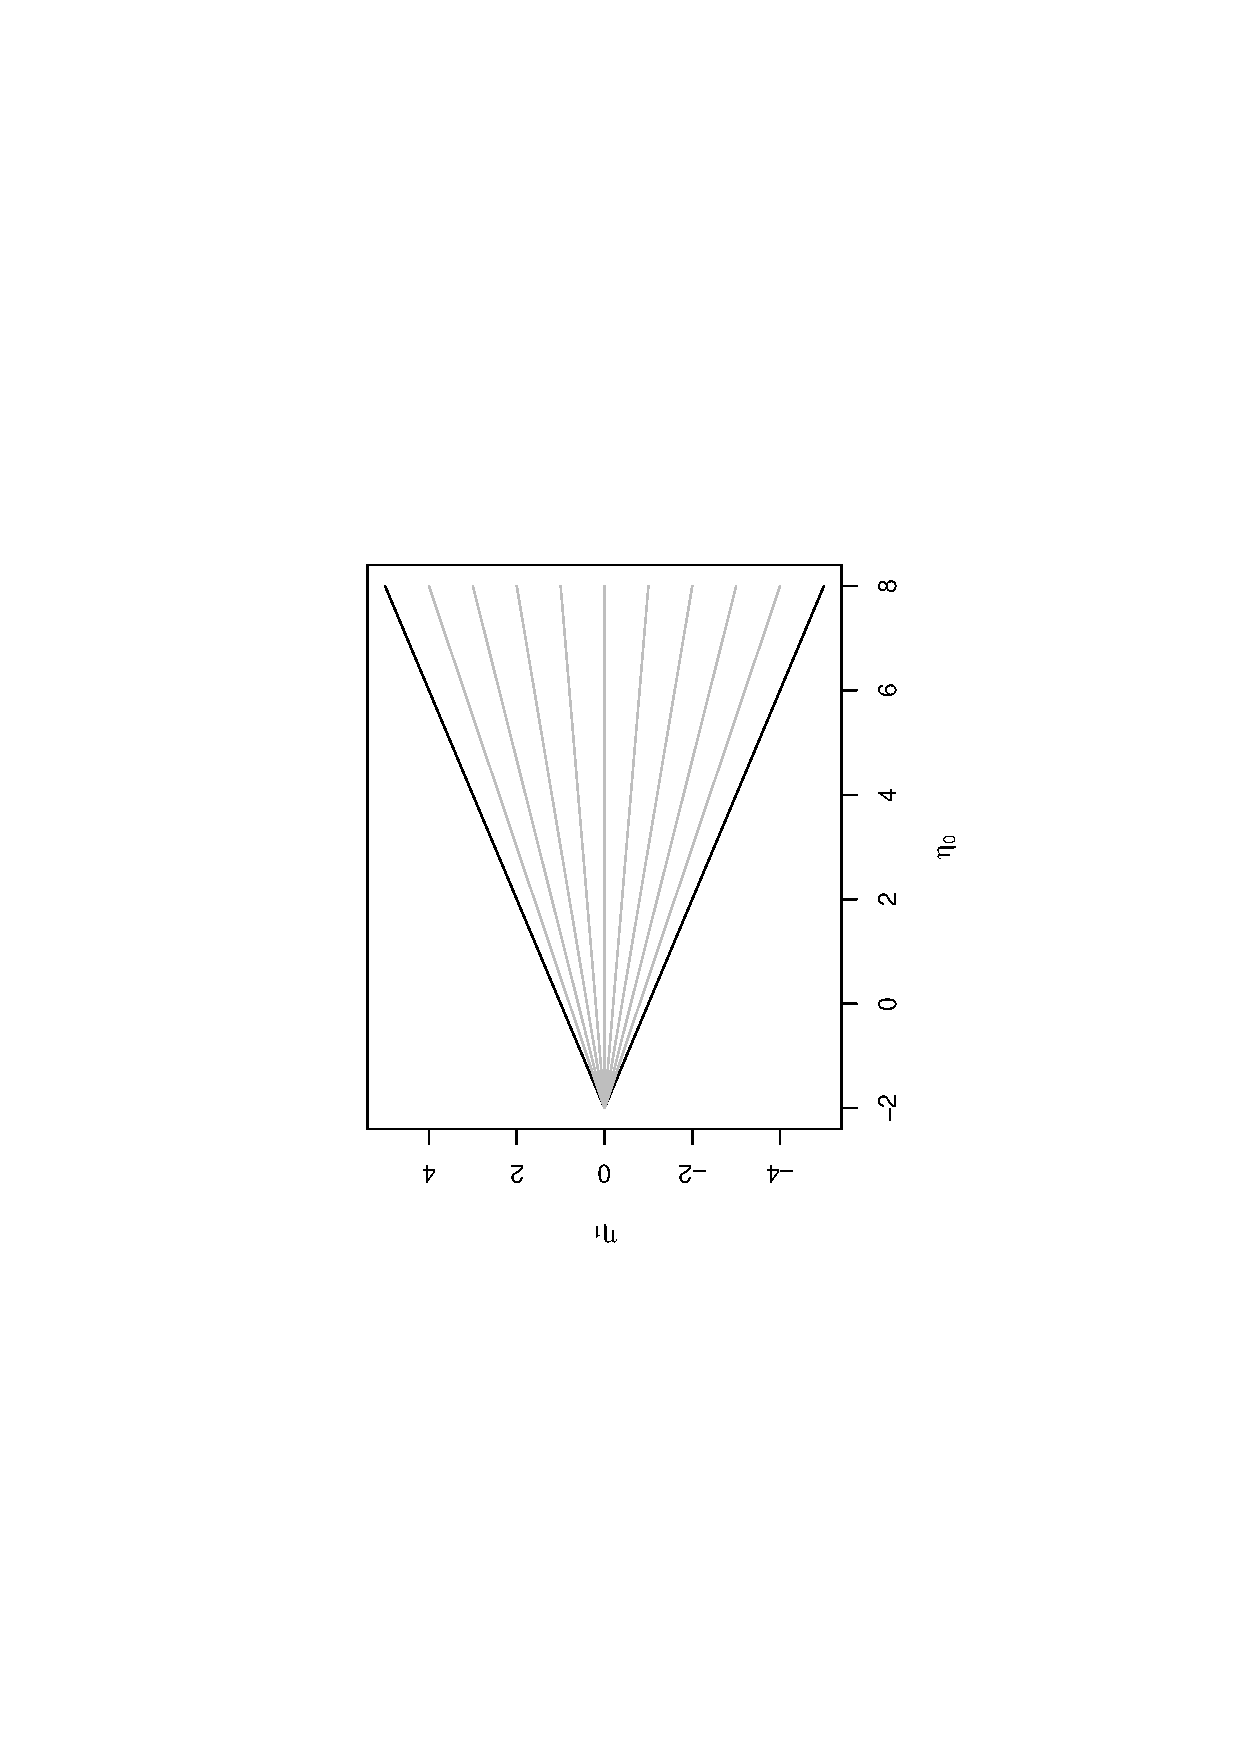
\includegraphics[trim = 80mm 45mm 80mm 60mm, clip, width=0.7\textwidth]{R/boatshape-domain}
\caption[Bounds for the domain of $\eta_0$ and $\eta_1$ for the Beta-Binomial model,
with rays of constant expectation for $y_c = \{0.1,0.2,\ldots,0.9\}$.]%
{Bounds for the domain of $\eta_0$ and $\eta_1$ for the Beta-Binomial model (black),
with rays of constant expectation for $y_c = \{0.1,0.2,\ldots,0.9\}$ (grey).}
\label{fig:boatshape-domain}
\end{figure}

As we wrote in Section~\ref{sec:concluding-outlook},
$\eta_1$ cannot have the convenient property of being equal to
the expectation of the mean sample statistic $\ttau(\x)$ (here, $s/n$),
as was the case for $y$.%
\footnote{For $\yz$, it holds that $\yz = \E\big[\E[\ttau(\x) \mid \psi] \mid \nz, \yz\big]$,
as mentioned in Section~\ref{sec:regularconjugates}.}
However, from \eqref{eq:trafotony} we can derive that coordinates $(\eta_0,\eta_1) \in \Eta$ satifying
\begin{align}
\label{eq:raysofconstantexpectation}
\eta_1 = f(\eta_0) &= (\eta_0 + 2)(y_c - \frac{1}{2}) 
\end{align}
will have a constant expectation $y_c$.
The domain $\Eta$, and these \emph{rays of constant expectation} emanating from the coordinate $(-2,0)$,
are depicted in Figure~\ref{fig:boatshape-domain}.

\subsection{The Boatshape}
\label{sec:boatshape-2}

When Mi\c{k}elis Bickis presented this parametrisation of conjugate priors at a talk,
both Frank Coolen and the author of this thesis had independently the same basic idea
for a set shape that allows for both \pdc\ sensitivity
%and gives `bonus precision' if prior and data agree especially well,
and more precise inferences in case of strong prior-data agreement.
The basic idea for this shape is described informally below,
while a suggestion for a parametrisation of such a shape is described and discussed
in the later subsections.

\subsubsection{Informal Rationale for Boat-Shaped Parameter Sets}
\label{boatshape-rationale}

In the parametrisation in terms of $(\nz,\yz)$ and $(\nn, \yn)$,
posterior inferences become more precise,
because the stretch in the main parameter dimension $y$, denoted by $\Delta_y(\PN)$,
tends to $0$ for $n \to \infty$ (see the discussion in Section~\ref{sec:gbicp-properties-criteria}).
In the domain $\Eta$ as depicted in Figure~\ref{fig:boatshape-domain},
instead the rays of constant expectation fan out for growing $n$, %**move outwards to the right,
while a parameter set will retain its size in updating.
Increased precision in a posterior parameter set $\EN$, which is just
its prior counterpart $\EZ$ shifted to the right,
is given by the fact the more $\EN$ is located to the right,
the fewer rays of constant expectation $\EN$ will intercept.
Imprecision in terms of $\E\big[\E[\ttau(\x) \mid \psi] \mid \nn, \yn\big] = \yn$
can thus be imagined as the size of the `shadow' that a set $\EN$ casts
when considering a light source in $(-2,0)$ (the point from which the rays of constant expectation emanate).
In short, the smaller this shadow, the more precise the inferences.

In the context of the model from Section~\ref{sec:miksworld},
we will denote by $\ynl$ and $\ynu$ the bounds of this shadow,
i.e.,
\begin{align*}
\ynl &:= \min_{(\ezn,\eon) \in \EN} \yn = \min_{(\ezn,\eon) \in \EN} \frac{\eon}{\ezn+2} + \frac{1}{2}\,, \\
\ynu &:= \max_{(\ezn,\eon) \in \EN} \yn = \max_{(\ezn,\eon) \in \EN} \frac{\eon}{\ezn+2} + \frac{1}{2}\,,
\end{align*}
and we call the coordinates $\argmin_{(\eta_0,\eta_1) \in \EN} \yn$ and $\argmax_{(\eta_0,\eta_1) \in \EN} \yn$
the \emph{touchpoints} of $\EN$ responsible for the shadow $[\ynl, \ynu]$.
Mutatis mutandis, the same definitions can be made for the prior set $\EZ$.

Due to the fanning out of rays, most shapes for $\EZ$ will lead to decreasing imprecision for increasing $n$.
Indeed, models of type~(\ref{enum:modeltypes-a}) from Section~\ref{sec:basicsetting},
where $\PZ = \nz \times [\yzl, \yzu]$,
are represented here again by a line segment $\EZ = \ezz \times [\eozl,\eozu]$,
such that the posterior touchpoints are, for any $s$ and $n$, $(\ezn,\eonl)$ and $(\ezz,\eonu)$,
where $\eonl$ and $\eonu$ are the updated versions of $\eozl$ and $\eozu$, respectively.
Due to \eqref{eq:eta-update}, it holds that $\eonu-\eonl = \eozu-\eozl$;
therefore, imprecision decreases here because a line segment of fixed size
will cast a smaller shadow when further to the right,
as illustrated in Figure~\ref{fig:boatshape-vertical}.

\begin{figure}  %trim=l b r t
\centering
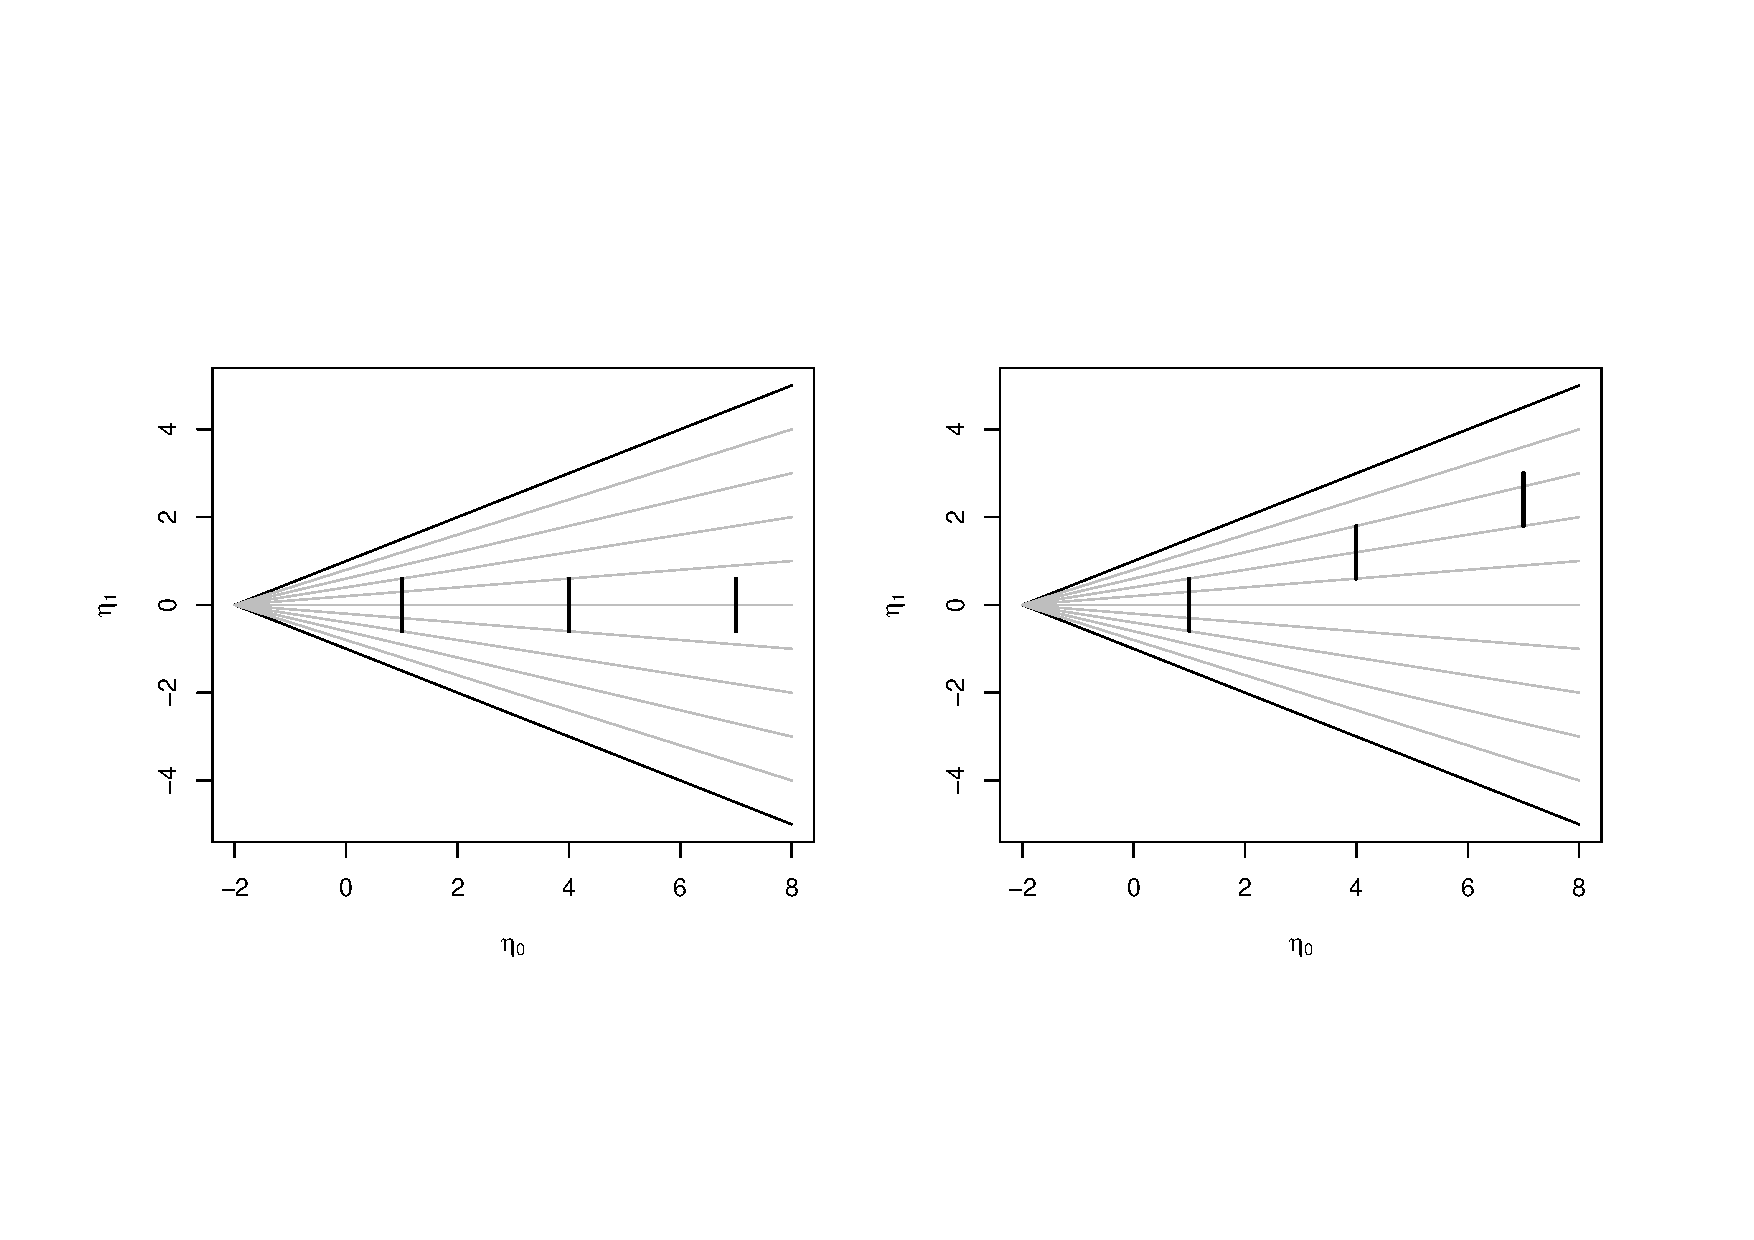
\includegraphics[trim = 15mm 45mm 25mm 60mm, clip, width=\textwidth]{R/boatshape-vertical}
\caption[Line segment parameter set $\EZ$ %
and respective posterior sets for $s/n=0.5$ and $s/n=0.9$.]%
{Parameter set $\EZ = \ezz \times [\text{\underline{$\eta$}${}_1\uz$},\eozu]$ and respective posterior sets $\EN$
for $s/n=0.5$ (left) and $s/n=0.9$ (right). Note that all sets have the same size,
imprecision decreasing only through their position on the $\eta_0$ axis.}
\label{fig:boatshape-vertical}
\end{figure}

For \pdc\ sensitivity, we need shapes that cover a range of $\eta_0$ values,
for the same reasons as in the framework of Section~\ref{sec:basicsetting},
where only sets with a range of $\nz$ values offered this property.
Sets that are elongated along the rays of constant expectation
will behave here similar to the rectangular shapes of Section~\ref{sec:basicsetting}.
When shifted along its respective ray of constant expectation,
imprecision will be reduced as the shadow of the set will become smaller just as described above for line segments.
When such a shape is instead shifted away from its ray of constant expectation,
imprecision will be increased, as a prolonged shape that is now turned away from its ray 
will cast a larger shadow.%
\footnote{This will become clear from the depiction of boatshape sets in Figure~\ref{fig:boatshape-posterior-mik}.} 

A set $\EZ$ allowing for less imprecison in case of strong prior-data agreement
must also be able to cast a smaller shadow if the update shift goes into the direction of its ray,
%of $s/n$ according the information,
but we will enhance this effect by considering now also the properties
of the canonical posteriors the coordinates of $\EN$ represent.

We have seen that for the conjugate distributions themselves,
$\nz$ is generally a parameter determining the spread of the distribution
(e.g., in the Normal-Normal model (see Section~\ref{sec:norm-norm}), $\nz$ was the inverse variance),
such that we will have more precise inferences if the shadow bounds $\ynl$ and $\ynu$
are attained at higher values of $\eta_0$, leading to lower variances in the
`critical' distributions at the boundary of the posterior expectation interval $[\ynl,\ynu]$.
For this to happen, we need a shape for which the touchpoints responsible for $\ynl$ and $\ynu$
are attained at higher values of $\eta_0$ in case of strong prior-data agreement.
Shapes that accomplish this must have a curvature along their length in the direction
of the constant rays of expectation.
The shape we suggest thus looks like a bullett, or like a boat with a transom stern
(see Figure~\ref{fig:boatshape-prior}).

\subsection{Basic Definition}
\label{sec:basicdefboat}

We will now present a parametrisation for such a boat-shaped parameter set $\EZ$.
To keep things simple, we will consider here and in the follwing only prior sets
that are symmetric around the $\eta_0$ axis, i.e., centered around $y_c = 0.5$,
expressing prior the information that we deem a fraction of successes of $\frac{s}{n} = \frac{1}{2}$
as the most probable.%
\footnote{The general case of sets $\EZ$ with central ray $y_c \neq 0.5$
is discussed informally in *****}

For the contours of $\EZ$, we suggest an exponential function as the functional form,
where the `prow' of the set is located at $(\ezl, 0)$.
The lower and the upper contour $\czl(\eta_0)$ and $\czu(\eta_0)$ are defined as
\begin{align*}
\czl(\eta_0) &= -a \left( 1 - e^{-b(\eta_0 - \ezl)} \right)\,, \\
\czu(\eta_0) &= \phantom{-}%
                 a \left( 1 - e^{-b(\eta_0 - \ezl)} \right)\,, 
\end{align*}
where $a$ and $b$ are parameters controlling the shape.
We will also need the respective derivations with respect to $\eta_0$, given by
\begin{align*}
\frac{d}{d\eta_0} \czl(\eta_0) &= -ab e^{-b(\eta_0 - \ezl)}\,, \\
\frac{d}{d\eta_0} \czu(\eta_0) &= \phantom{-}%
                                   ab e^{-b(\eta_0 - \ezl)}\,.
\end{align*}

For this basic situation, given the parameters $\ezl$, $\ezu$, $a$, and $b$,
$\EZ$ is thus defined as
\begin{align*}
\EZ =
\{(\eta_0,\eta_1) \colon \ezl \le \eta_0 \le \ezu, \czl(\eta_0) \le  \eta_1 \le \czu(\eta_0) \}\,.
\end{align*}
A prior boatshape set with $\ezl=1$, $\ezu=6$, $a=2$, and $b=0.8$ is depicted in Figure~\ref{fig:boatshape-prior},
where the left graph shows this set as defined in terms of $(\eta_0,\eta_1)$,
and the right graph shows the set from the left transformed into the space $\N \times \Y$.

\begin{figure}  %trim=l b r t
\centering
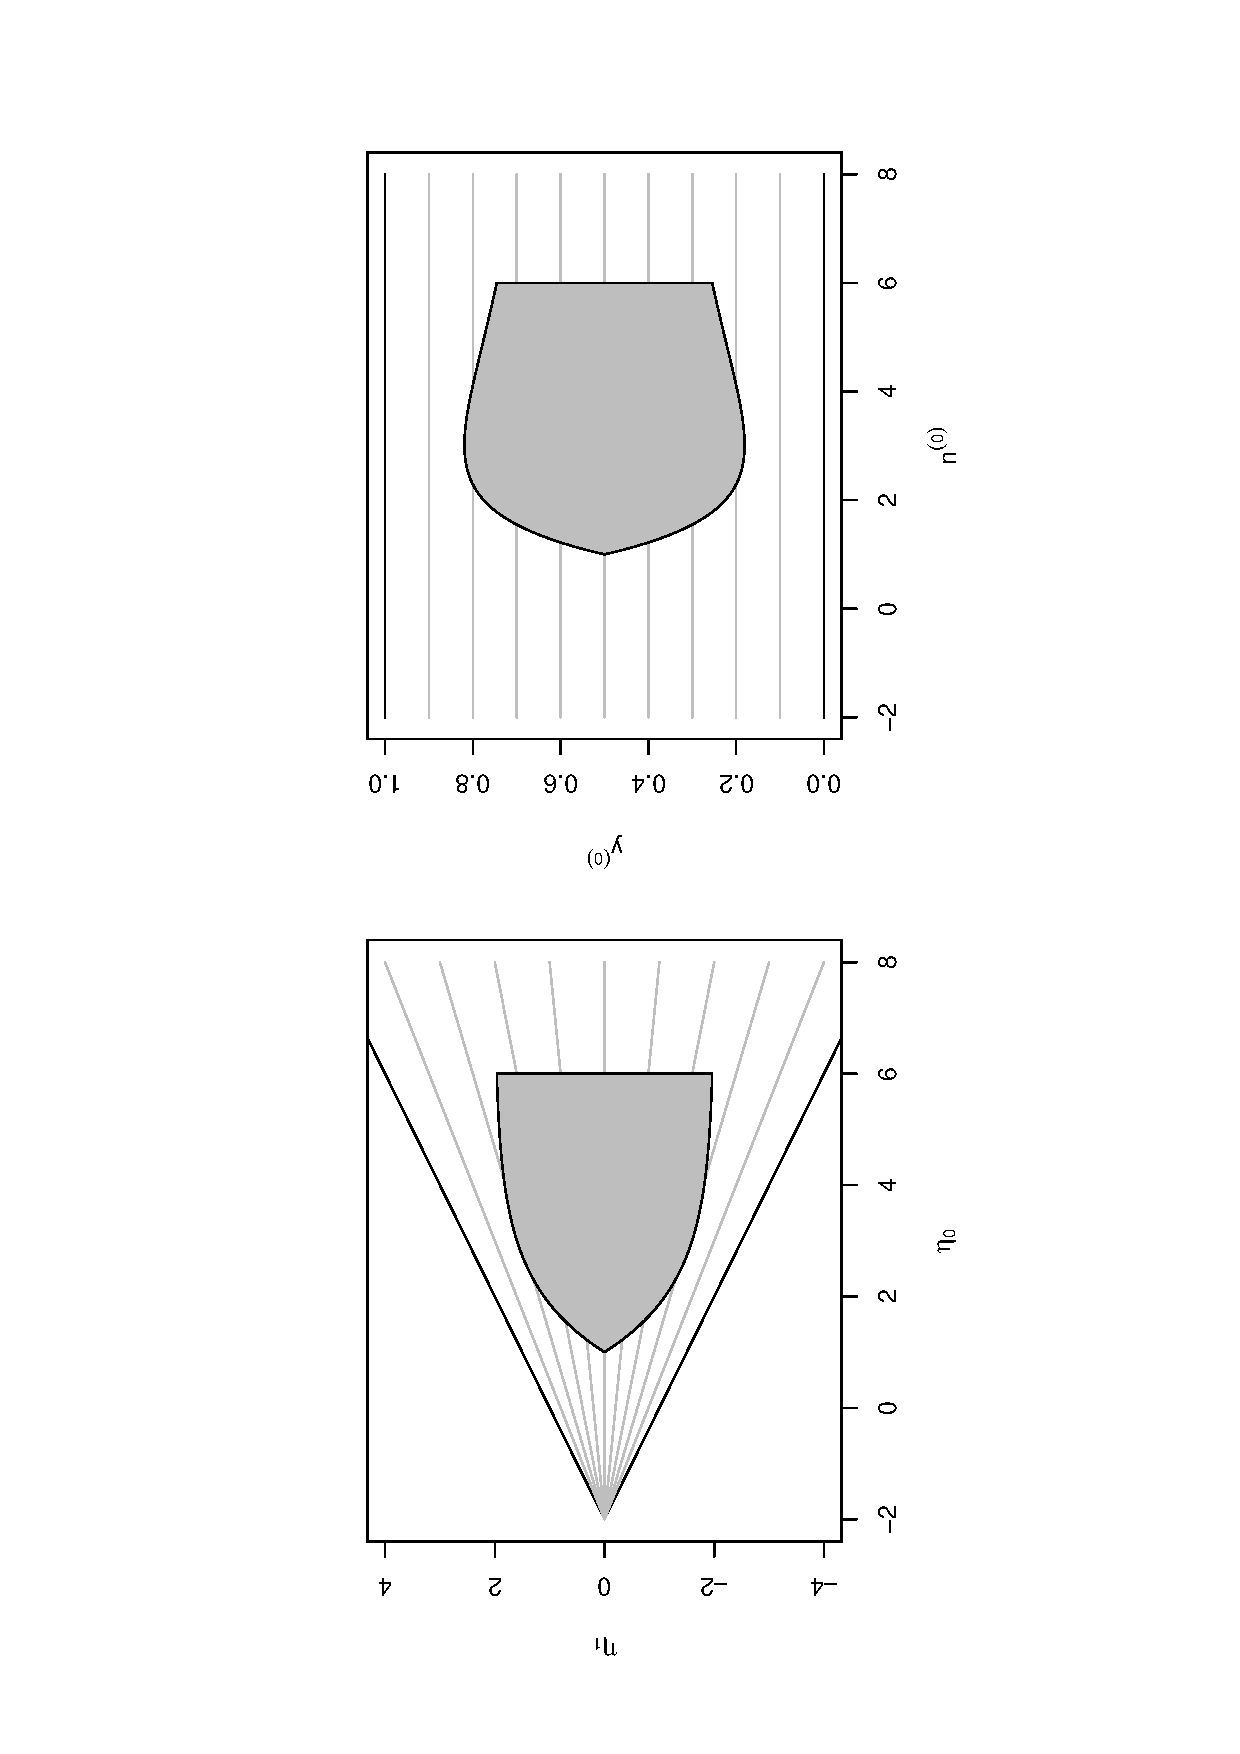
\includegraphics[trim = 15mm 45mm 25mm 60mm, clip, width=\textwidth]{R/boatshape-prior}
\caption[Boatshape prior set in the parametrisation via $(\eta_0,\eta_1)$ and via $(\nz,\yz)$.]%
{Boatshape prior set in the parametrisation via $(\eta_0,\eta_1)$ (left) and via $(\nz,\yz)$ (right),
with parameters $\ezl=1$, $\ezu=6$, $a=2$, and $b=0.8$.}
\label{fig:boatshape-prior}
\end{figure}


We have as yet no good formal description for the role of the parameters $a$ and $b$. %that,
%togeher with $\ezl$ and $\ezu$, define the boat-set (see Section~\ref{sec:basicdefboat} below).
Informally, $a$ determines the half-width of the set;
the width, i.e., the size in the $\eta_1$ dimension, would be $a$ if $\ezu \to \infty$.
$b$ instead determines the `bulkyness' of the shape.
Together with $\ezl$, $a$ and $b$ determine the prior interval for the expected success probability $[\yzl, \yzu]$.
For fixed $\ezl$ and $a$, increasing $b$ leads to a wider prior expectation interval.
For $[\yzl, \yzu]$, the choice of $\ezu$ is irrelevant.%
\footnote{$\ezu$ plays only a role in determining when the `unhappy learning' phase starts
(see end of Section~\ref{sec:generalupdate}).}


\begin{figure}  %trim=l b r t
\centering
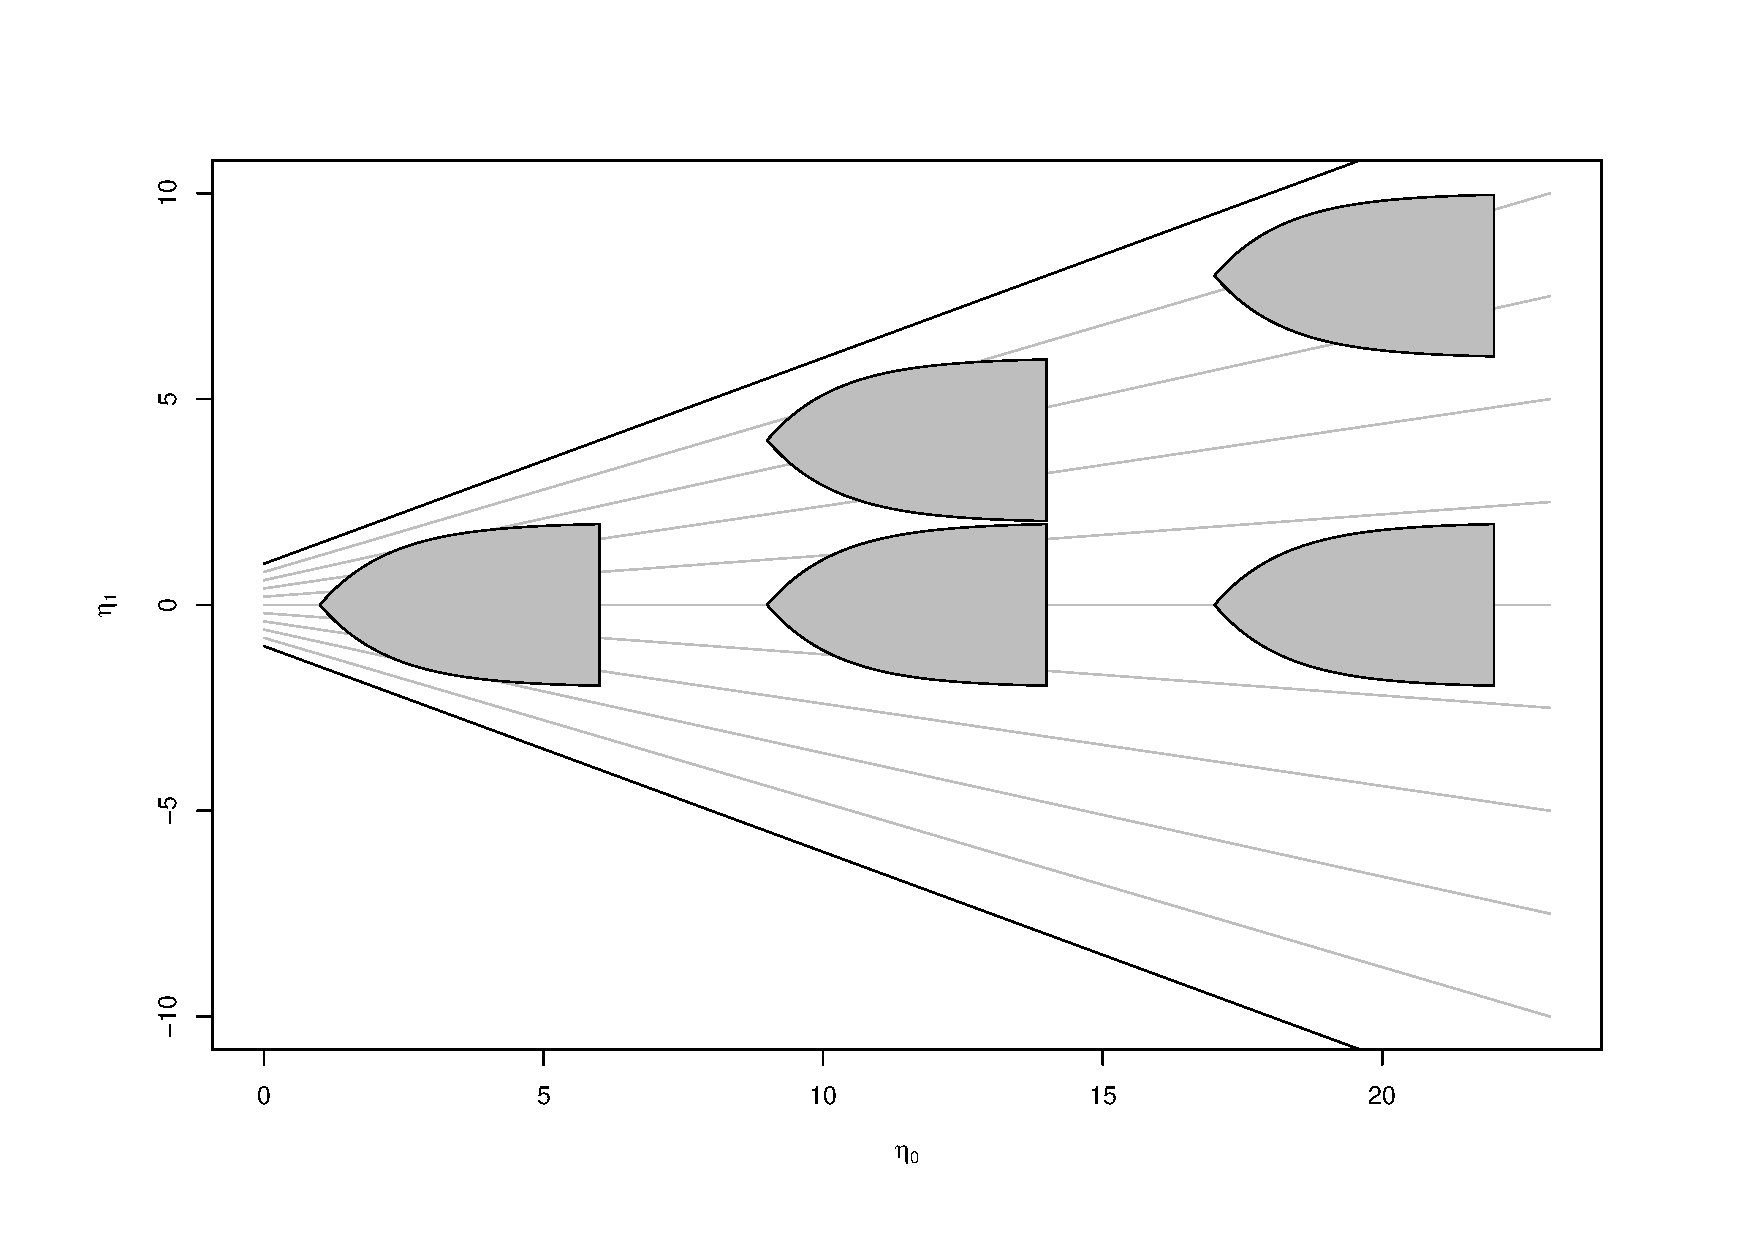
\includegraphics[trim = 15mm 10mm 25mm 25mm, clip, width=\textwidth]{R/boatshape-posterior-mik}
\caption[Boatshape prior and posterior sets for data in accordance and in conflict with the prior.]%
{Boatshape prior and posterior sets for data in accordance and in conflict with the prior.
The prior set is the same as in Figure~\ref{fig:boatshape-prior}.
While the posterior sets for $\frac{s}{n}=0.5$ move along the ray for $y_c=0.5$,
the posterior sets for $\frac{s}{n}=1$ are shifted away from the ray for $y_c=0.5$,
resulting in increased posterior imprecision.
Note that lower and upper touchpoints are in the middle of the contour
for the prior and the posterior resulting for data $\frac{s}{n}=\frac{4}{8}$,
while at least one touchpoint is at the end for all other sets.
(see also Figure~\ref{fig:boatshape-posterior-normal}).}
\label{fig:boatshape-posterior-mik}
\end{figure}


\begin{figure}  %trim=l b r t
\centering
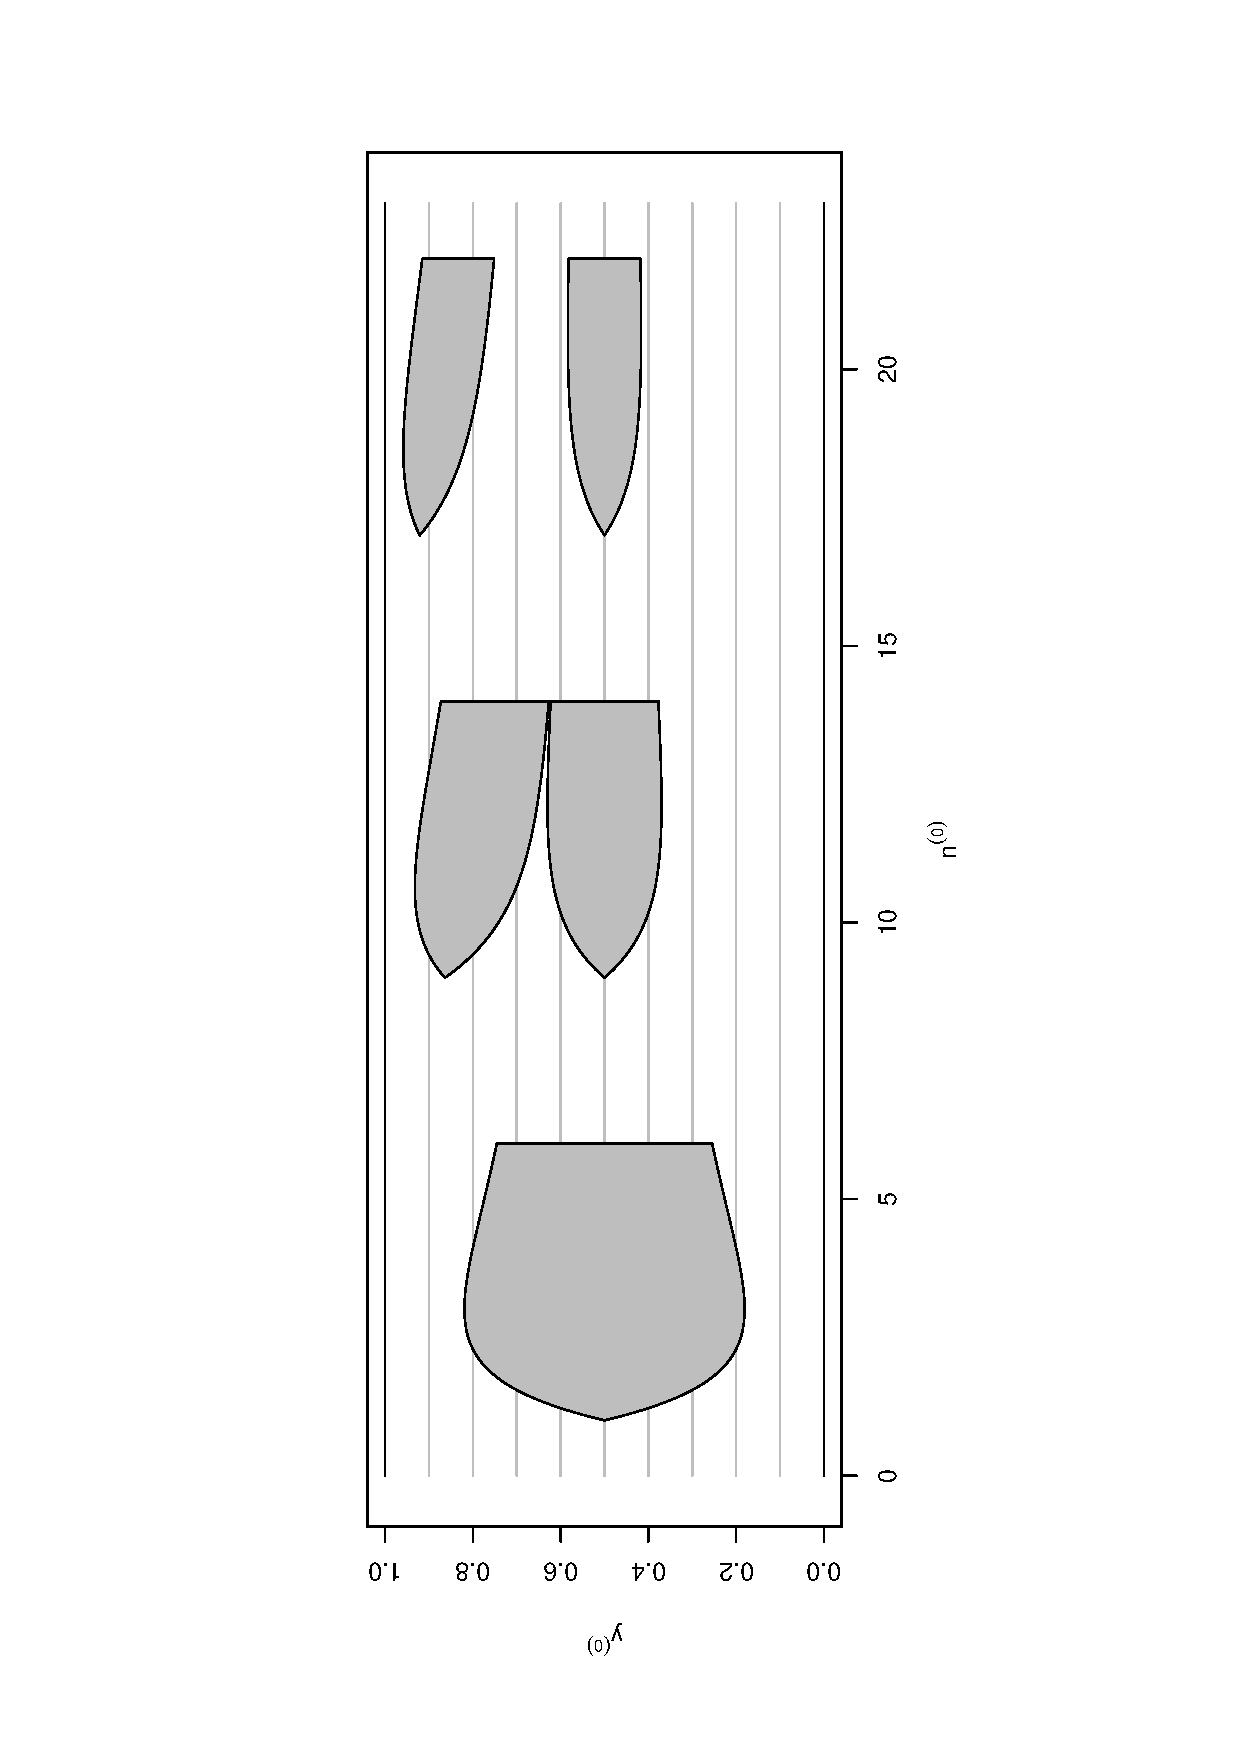
\includegraphics[trim = 15mm 45mm 25mm 60mm, clip, width=\textwidth]{R/boatshape-posterior-normal}
\caption[Boatshape prior and posterior sets from Figure~\ref{fig:boatshape-posterior-mik} in the parametrisation via $(\nz,\yz)$.]%
{Boatshape prior and posterior sets from Figure~\ref{fig:boatshape-posterior-mik} in the parametrisation via $(\nz,\yz)$.
Note that in the strong prior-data agreement case,
posteriors based on a rectangular set with the same prior main parameter imprecision
would be larger than the ones depicted here, illustrating the extra gain in precision.}
\label{fig:boatshape-posterior-normal}
\end{figure}


--------------------------------


possible to put information in near-noninformative set $\EZ$!

***As our preliminary studies show some very appealing results in case of the Beta-Binomial model,
for which a possible parametrisation of our shape is discussed in Section~\ref{sec:boatshape},
we are confident that these encouraging results also hold for the Normal-Normal model
and in the general case of canonical conjugates.
A joint publication of Mi\c{k}elis Bickis, Frank Coolen and the author of this thesis is planned
that will elaborate these findings in more detail.





%
